%\documentclass[12pt,serif]{beamer}
%\documentclass[tikz,12pt,svgnames]{beamer}

%For printing
%\documentclass[table,handout,tikz,12pt,svgnames]{beamer}
%With animations
\documentclass[table,tikz,12pt,svgnames]{beamer}

\usepackage{CM-preamble}
\usepackage{gitdags}
\usepackage{subcaption}

\definecolor{darkgreen}{rgb}{0,0.6,0}
\definecolor{red}{rgb}{1,0,0}
\definecolor{green}{rgb}{0,1,0}
\definecolor{blue}{rgb}{0,0,1}
\definecolor{cyan}{rgb}{0.4,1,1}
\definecolor{orange}{rgb}{1,0.7,0}
\definecolor{dkgreen}{rgb}{0,0.6,0}
\definecolor{gray}{rgb}{0.5,0.5,0.5}
\definecolor{purple}{rgb}{0.58,0,0.82}
\definecolor{mintedbackground}{rgb}{0.95,0.95,0.95}
 
\title{\LARGE Gestion de versions}
\subtitle{avec \texttt{git}}
\date{}

%README TODO STUFF

\begin{document}

%%%%%%%%%%% ANIMATION Branch 2
\begin{frame}[fragile]
\frametitle{The DAG in Git: Branches 2}
\only<1>{
	\begin{figure}
		\begin{subfigure}[h]{\textwidth}
			%\centering
			\begin{tikzpicture}
			% Commit DAG
			\gitDAG[grow right sep = 2em]{
				27ff4 -- 31490 -- ab5d1 -- ffd5c -- 8a928
			};
			% Tag reference
			%	\gittag [v0p1] {v0.1} {above=of A} {A}
			% Remote branch
			% Branch
			\gitbranch
			{master}     % node name and text 
			{above=of ab5d1} % node placement
			{ab5d1}          % target
			% HEAD reference
			\gitHEAD
			{below=of 8a928} % node placement
			%			{right=of legumes} % node placement
			{8a928}          % target
			\gitbranch {legumes} {above=of 8a928} {8a928}
			
			\end{tikzpicture}
			\subcaption{Travaillons sur \texttt{master}}
			\only<2>{$\Longrightarrow$ \texttt{legumes.txt} n'existe plus dans \textit{Working Directory})}
		\end{subfigure}
	\end{figure}
}

\only<2-3>{
	\begin{figure}
		\begin{subfigure}[h]{\textwidth}
			%\centering
			\begin{tikzpicture}
			% Commit DAG
			\gitDAG[grow right sep = 2em]{
				27ff4 -- 31490 -- ab5d1 -- ffd5c -- 8a928
			};
			% Tag reference
			%	\gittag [v0p1] {v0.1} {above=of A} {A}
			% Remote branch
			% Branch
			\gitbranch
			{master}     % node name and text 
			{above=of ab5d1} % node placement
			{ab5d1}          % target
			% HEAD reference
			\gitHEAD
			{below=of ab5d1} % node placement
			%			{right=of legumes} % node placement
			{ab5d1}          % target
			\gitbranch {legumes} {above=of 8a928} {8a928}
			
			\end{tikzpicture}
			\subcaption{Travaillons sur \texttt{master}}
			\only<2>{$\Longrightarrow$ \texttt{legumes.txt} n'existe plus dans \textit{Working Directory})}
			\vspace{0.33em}
		\end{subfigure}
	\end{figure}
}

\only<4>{
	\begin{figure}
		\begin{subfigure}[h]{\textwidth}
			%\centering
			\begin{tikzpicture}
			% Commit DAG
			\gitDAG[grow right sep = 2em]{
				27ff4 -- 31490 -- ab5d1 -- {ffd5c -- 8a928, 21721}
			};
			% Tag reference
			%	\gittag [v0p1] {v0.1} {above=of A} {A}
			% Remote branch
			% Branch
			\gitbranch
			{master}     % node name and text 
			{below=of 21721} % node placement
			{21721}          % target
			% HEAD reference
			\gitHEAD
			{right=of master} % node placement
			%			{right=of legumes} % node placement
			{21721}          % target
			\gitbranch {legumes} {above=of 8a928} {8a928}
			
			\end{tikzpicture}
			\subcaption{Après nouveau \textit{commit} sur \texttt{master}}
			\only<2>{$\Longrightarrow$ \texttt{legumes.txt} n'existe plus dans \textit{Working Directory})}
			\vspace{-3em}
		\end{subfigure}
	\end{figure}
}

%\vspace{-0.5cm}
%\only<2-3>{
%\begin{block}{Sur le terminal \ldots}
%\pause[2]
%\vspace{-0.2cm}
\vspace{0.4cm} \begin{center} \noindent\makebox[\linewidth]{\line(2,0){500}} \end{center} \vspace{-0.4cm}
\begin{minted}[mathescape=true,escapeinside=||,tabsize=4,fontsize=\footnotesize,]{c}
	git checkout master
\end{minted}

\only<1>{\begin{tikzpicture}[remember picture,overlay]\node[xshift=1cm,yshift=2.6cm] at (current page.south west) {$\hookrightarrow$};\end{tikzpicture}}
\only<2>{\begin{tikzpicture}[remember picture,overlay]\node[xshift=1cm,yshift=2cm] at (current page.south west) {$\hookrightarrow$};\end{tikzpicture}}
\pause[3]
\begin{minted}[mathescape=true,escapeinside=||,tabsize=4,fontsize=\footnotesize,]{c}
	echo poire |>{}>| fruits.txt ; git add fruits.txt
	git commit -m "Ajouté poire à fruits.txt"
	  |$\longrightarrow$| ID = 21721
\end{minted}
\only<3>{\begin{tikzpicture}[remember picture,overlay]\node[xshift=1cm,yshift=2cm] at (current page.south west) {$\hookrightarrow$};\end{tikzpicture}}
\only<4->{\begin{tikzpicture}[remember picture,overlay]\node[xshift=1cm,yshift=0.6cm] at (current page.south west) {$\hookrightarrow$};\end{tikzpicture}}
\end{frame}
%%%%%%%%%%% End ANIMATION Branch 2


%%%%%%%%%%% ANIMATION Merge 1
\begin{frame}[fragile]
\frametitle{The DAG in Git: Merge 1}
\only<1-2>{
	\begin{figure}
		\begin{subfigure}[h]{\textwidth}
			%\centering
			\begin{tikzpicture}
			% Commit DAG
			\gitDAG[grow right sep = 1.5em]{
				27ff4 -- 31490 -- ab5d1 -- {ffd5c -- 8a928, 21721}
			};
			% Tag reference
			%	\gittag [v0p1] {v0.1} {above=of A} {A}
			% Remote branch
			% Branch
			\gitbranch
			{master}     % node name and text 
			{below=of 21721} % node placement
			{21721}          % target
			% HEAD reference
			\gitHEAD
			{right=of legumes} % node placement
			%			{right=of legumes} % node placement
			{8a928}          % target
			\gitbranch {legumes} {above=of 8a928} {8a928}
			
			\end{tikzpicture}
			\subcaption{Allons sur \texttt{légumes}, regardons les différences}
			%\only<2>{$\Longrightarrow$ \texttt{legumes.txt} n'existe plus dans \textit{Working Directory})}
		\end{subfigure}
	\end{figure}
}

\only<3>{
	\begin{figure}
		\begin{subfigure}[h]{\textwidth}
			%\centering
			\begin{tikzpicture}
			% Commit DAG
			\gitDAG[grow right sep = 1.5em]{
				27ff4 -- 31490 -- ab5d1 -- {ffd5c -- 8a928, 21721} -- 760cf
			};
			% Tag reference
			%	\gittag [v0p1] {v0.1} {above=of A} {A}
			% Remote branch
			% Branch
			\gitbranch
			{master}     % node name and text 
			{below=of 21721} % node placement
			{21721}          % target
			% HEAD reference
			\gitHEAD
			{above=of 760cf} % node placement
			%			{right=of legumes} % node placement
			{760cf}          % target
			\gitbranch {legumes} {left=of gitHEAD} {760cf}
			
			\end{tikzpicture}
			\subcaption{Merger \texttt{master} dans \texttt{légumes} : produit un \underline{nouveau commit}}
			%\only<2>{$\Longrightarrow$ \texttt{legumes.txt} n'existe plus dans \textit{Working Directory})}
		\end{subfigure}
	\end{figure}
}


%\vspace{-0.5cm}
%\only<2-3>{
%\begin{block}{Sur le terminal \ldots}
%\pause[2]
%\vspace{-0.2cm}
\vspace{0.4cm} \begin{center} \noindent\makebox[\linewidth]{\line(2,0){500}} \end{center} \vspace{-0.4cm}
\begin{minted}[mathescape=true,escapeinside=||,tabsize=4,fontsize=\footnotesize,]{c}
git checkout legumes
\end{minted}
\pause[2]
\begin{minted}[mathescape=true,escapeinside=||,tabsize=4,fontsize=\footnotesize,]{c}
git diff master
\end{minted}
\pause[3]
\begin{minted}[mathescape=true,escapeinside=||,tabsize=4,fontsize=\footnotesize,]{c}
git merge master
\end{minted}
\end{frame}
%%%%%%%%%%% End ANIMATION Merge 1

\begin{frame}
\frametitle{Merge 1 : Vue dans la console}
%\begin{block}{Représentation par pointeurs}%Parcours postfixé ou \texttt{GRD}}
\begin{adjustwidth}{-1cm}{-0.8cm}{}
	\begin{center}
		{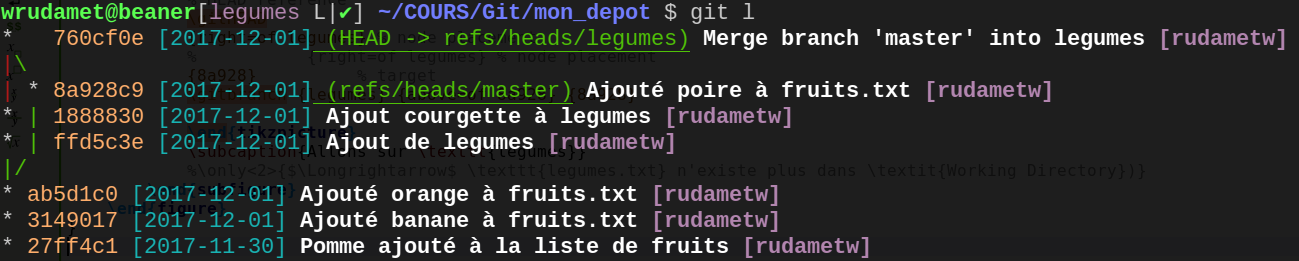
\includegraphics[scale=0.3]{images/git_log_merge.png}}
	\end{center}
\end{adjustwidth}
%\end{block}
\end{frame}



%%%%%%%%%%% ANIMATION Merge 2
\begin{frame}[fragile]
\frametitle{The DAG in Git: Merge 2}
\only<1>{
	\begin{figure}
		\begin{subfigure}[h]{\textwidth}
			%\centering
			\begin{tikzpicture}
			% Commit DAG
			\gitDAG[grow right sep = 1.5em]{
				27ff4 -- 31490 -- ab5d1 -- {ffd5c -- 8a928, 21721} -- 760cf
			};
			% Tag reference
			%	\gittag [v0p1] {v0.1} {above=of A} {A}
			% Remote branch
			% Branch
			\gitbranch
			{master}     % node name and text 
			{below=of 21721} % node placement
			{21721}          % target
			% HEAD reference
			\gitHEAD
			{right=of master} % node placement
			%			{right=of legumes} % node placement
			{21721}          % target
			\gitbranch {legumes} {above=of 760cf} {760cf}
			
			\end{tikzpicture}
			\subcaption{Allons sur \texttt{master}}
			%\only<2>{$\Longrightarrow$ \texttt{legumes.txt} n'existe plus dans \textit{Working Directory})}
		\end{subfigure}
	\end{figure}
}

\only<2>{
	\begin{figure}
		\begin{subfigure}[h]{\textwidth}
			%\centering
			\begin{tikzpicture}
			% Commit DAG
			\gitDAG[grow right sep = 1.5em]{
				27ff4 -- 31490 -- ab5d1 -- {ffd5c -- 8a928, 21721} -- 760cf
			};
			% Tag reference
			%	\gittag [v0p1] {v0.1} {above=of A} {A}
			% Remote branch
			% Branch
			\gitbranch
			{master}     % node name and text 
			{below=of 760cf} % node placement
			{760cf}          % target
			% HEAD reference
			\gitHEAD
			{left=of legumes} % node placement
			%			{right=of legumes} % node placement
			{760cf}          % target
			\gitbranch {legumes} {above=of 760cf} {760cf}
			
			\end{tikzpicture}
			\subcaption{Merger \texttt{légumes} dans \texttt{master} : \underline{pas de nouveau commit}}
			%\only<2>{$\Longrightarrow$ \texttt{legumes.txt} n'existe plus dans \textit{Working Directory})}
		\end{subfigure}
	\end{figure}
}

\only<3>{
	\begin{figure}
		\begin{subfigure}[h]{\textwidth}
			%\centering
			\begin{tikzpicture}
			% Commit DAG
			\gitDAG[grow right sep = 1.5em]{
				27ff4 -- 31490 -- ab5d1 -- {ffd5c -- 8a928, 21721} -- 760cf
			};
			% Tag reference
			%	\gittag [v0p1] {v0.1} {above=of A} {A}
			% Remote branch
			% Branch
			\gitbranch
			{master}     % node name and text 
			{below=of 760cf} % node placement
			{760cf}          % target
			% HEAD reference
			\gitHEAD
			{above=of 760cf} % node placement
			%			{right=of legumes} % node placement
			{760cf}          % target
%			\gitbranch {legumes} {above=of 760cf} {760cf}
			
			\end{tikzpicture}
			\subcaption{Effacer la branche \texttt{légumes}}
			%\only<2>{$\Longrightarrow$ \texttt{legumes.txt} n'existe plus dans \textit{Working Directory})}
		\end{subfigure}
	\end{figure}
}
\vspace{0.4cm} \begin{center} \noindent\makebox[\linewidth]{\line(2,0){500}} \end{center} \vspace{-0.4cm}

\begin{minted}[mathescape=true,escapeinside=||,tabsize=4,fontsize=\footnotesize,]{c}
git checkout master
\end{minted}
\pause[2]
\begin{minted}[mathescape=true,escapeinside=||,tabsize=4,fontsize=\footnotesize,]{c}
git diff legumes
git merge legumes
\end{minted}
\pause
\begin{minted}[mathescape=true,escapeinside=||,tabsize=4,fontsize=\footnotesize,]{c}
git branch -d legumes
\end{minted}
\end{frame}
%%%%%%%%%%% End ANIMATION Merge 2


\end{document}
% % % % % % % % % % % % % % % % % % % % % % % % % % %
% END
% % % % % % % % % % % % % % % % % % % % % % % % % % %